\chapter{The Compact Muon Solenoid Experiment at the LHC}
\section{The Large Hadron Collider}
The Large Hadron Collider (LHC) is a circular synchrotron of circumference 27km designed to collide proton beams with a centre of mass energy $\sqrt{s}  = 14$\,TeV at a final design luminosity of $10^{34}$cm$^{-2}$s$^{-1}$, with the aim of discovering new physics at the TeV scale.Utilising the tunnel of the previous e+e- machine LEP, 


\section{The Compact Muon Solenoid}

The Compact Muon Solenoid (CMS) is one of the two multi-purpose detectors at the LHC, designed to capitalise on the full range of physics opportunities available at the LHC. These goals are pursued through the design and construction of the detector and development of software for the reconstruction of physics objects. The detector is constructed of several detector sub-systems contained inside and wrapped in layers around a central 13m long 4T super conducting solenoid as shown in Figure \ref{fig:CMS_Struct}. 

The detector is 21m long, 15m wide and weights 14000 t, and consists of five wheel-like barrel sections and two end-caps to close. In order for CMS to search for new physics among the high order of Standard Model backgrounds, it is of key importance to develop a detector which has impressive energy and momentum resolution, and particle identification. Different particles interact differently with matter and therefore a number of sub-detectors are needed in order to gather all the relative information. The path travelled by a particle from the interaction point involves the following regions. 

\begin{figure}
\centering
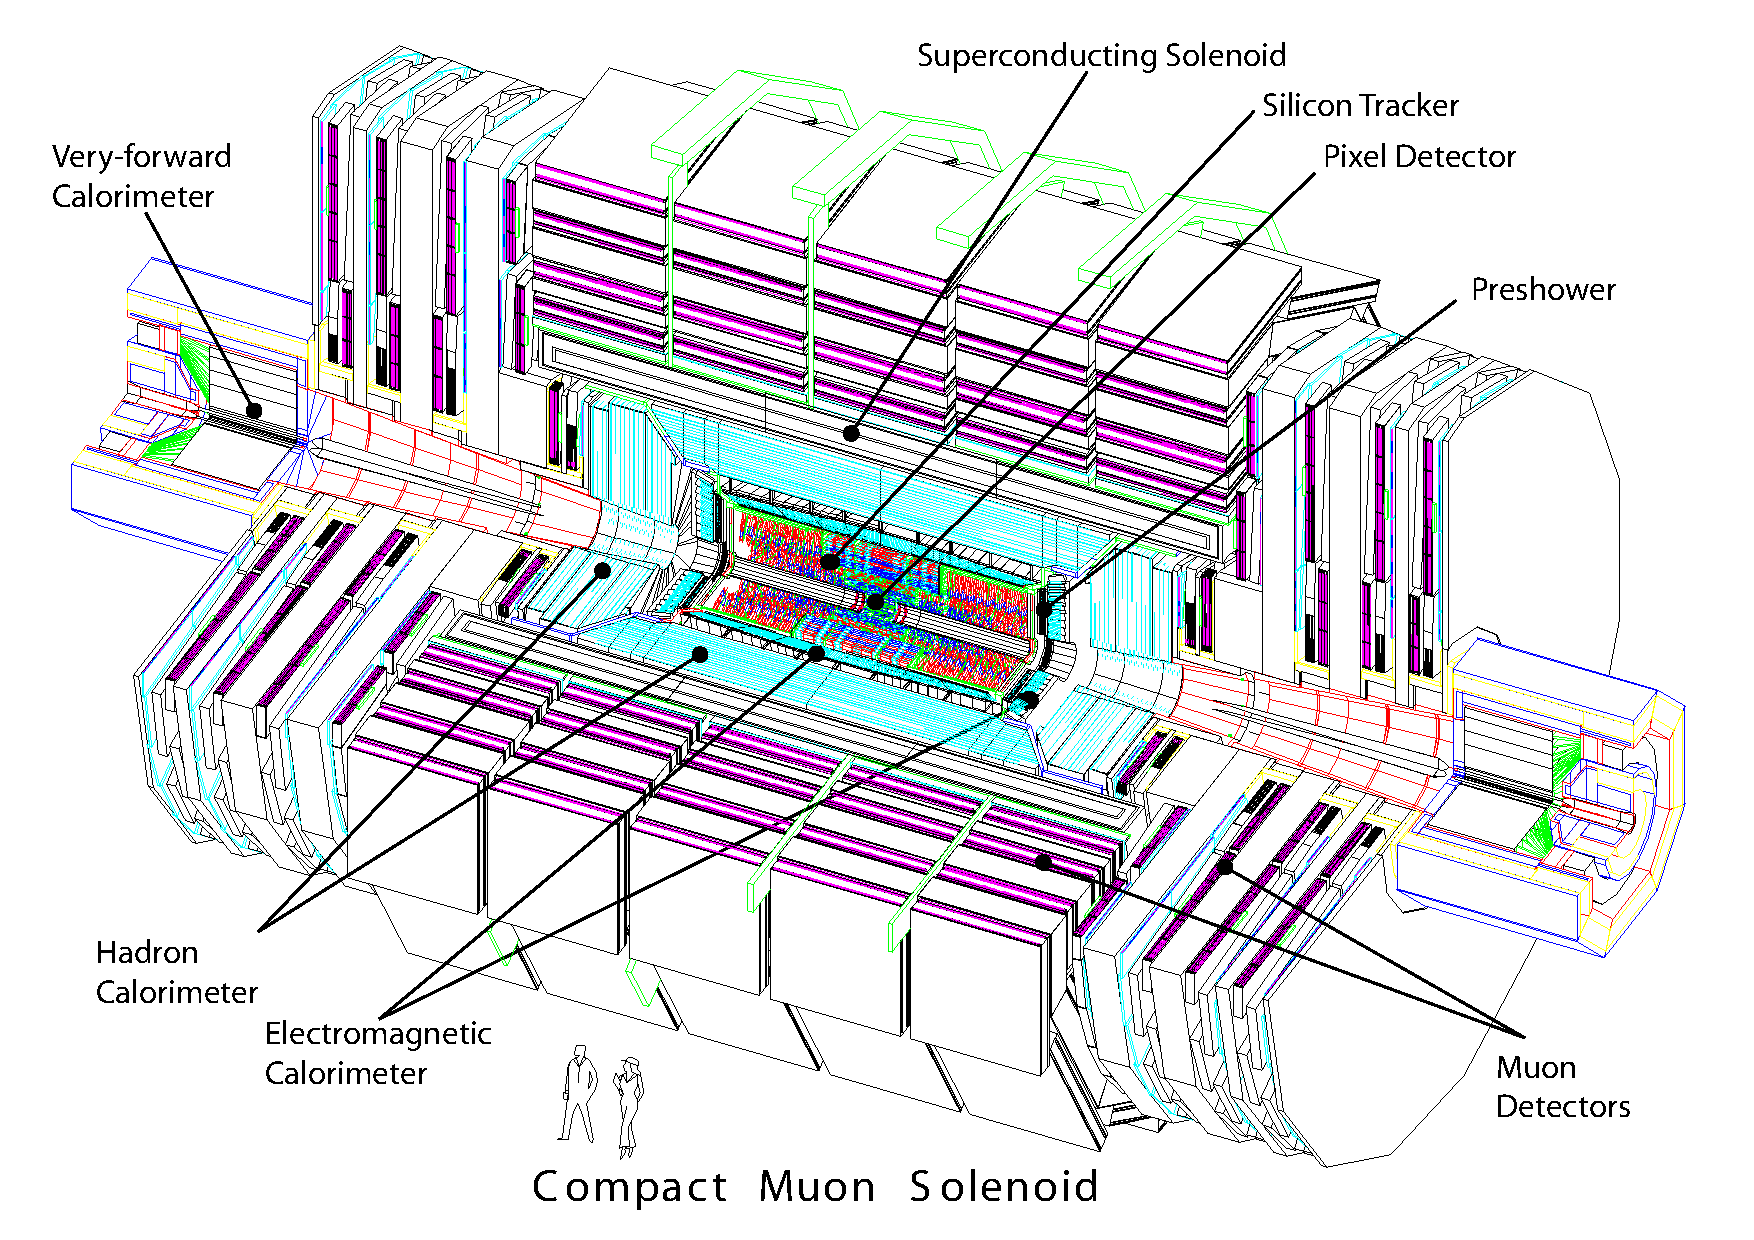
\includegraphics[width=0.8\textwidth]{Figures/Detector/CMS_Structure}
\caption{A cutaway diagram of the CMS detector structure identifying the main individual sub-systems.}
\label{fig:CMS_Struct}
\end{figure}

The high magnetic field was chosen in order to achieve the bending power necessary for good charged particle momentum resolution. The inner bore of the solenoid is large enough that the inner tracker and the calorimeters are located inside, which minimises the material the partials pass through before entering the calorimeters. This allows a good energy measurement. Four muon "stations" of aluminium drift tubes are integrates within the   iron magnetic field return yoke. The full design description can be found in the CMS Technical Design Proposal \cite{CMSTDP}. As different particles pass through the detector they interact in the sub-systems depending on their type. A transverse slice through the detector illustrating the path through the machine of each type of particle is shown in Figure \ref{fig:CMS_Slice} 





\begin{figure}
\centering
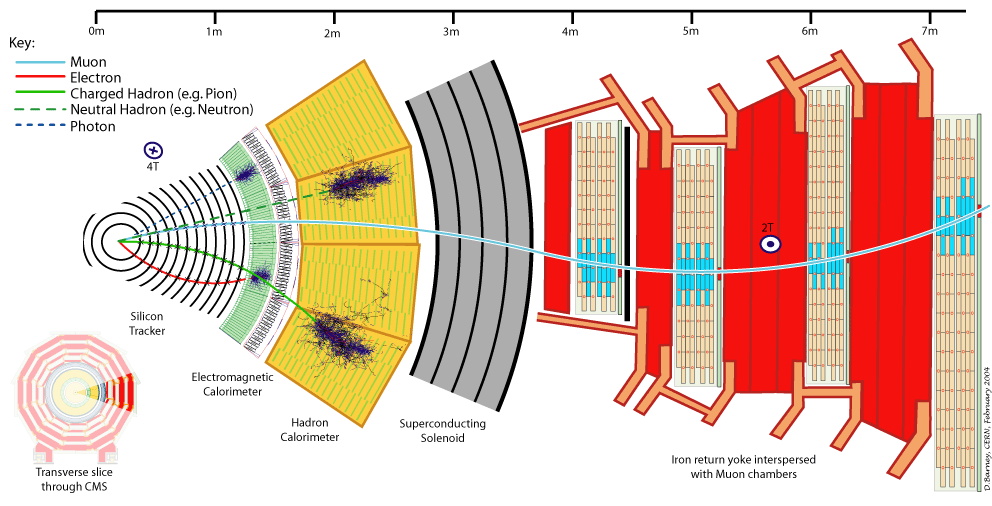
\includegraphics[width=0.8\textwidth]{Figures/Detector/CMS_Slice}
\caption{Transverse slice through the CMS Detector showing each type of particle and how it interacts with the sub-detectors.}
\label{fig:CMS_Slice}
\end{figure}
\subsection{Coordinate System}

The coordinate system chosen by CMS uses the nominal interaction point within the detector as the origin. The x-axis points radially inwards to the centre of the beam pipe, and the y-axis points vertically upward. The z-axis then points in the direction of the beam. The azimuthal angle $\phi$ is defined as the angle from the x-axis in the x-y plane, and the polar angle $\theta$ from the z-axis. However, it is common convention to express $\theta$ in terms of the Lorentz Invariant quantity, pseudorapidity~\begin{math}
\eta = -\ln \tan (\theta / 2) 
\end{math}, as particle production is approximately uniform in $\eta$. The transverse components of the energy and momentum, denoted $E_{T}$ and $p_{T}$ are then calculated form the $x$ and $y$ components. 
\subsection{Tracker}



The first sub-detector encountered by particles is the multi-layer silicon tracker, which records precise information about the path of charged particles bending under the magnetic field. It is placed as close to the interaction point as possible in order to distinguish the primary interaction from secondary vertices of particles with significant lifetimes. This is particularly important in the case of identifying B mesons, which can travel a measurable distance before decaying.  

The tracker is divided into regions defined by the radius r from the interaction point, as the expected particle flux decreases rapidly as the radius increases. This is due to the high magnetic field, which causes low momentum particles to have small radial helical trajectories.

Nearest to the primary vertex at 4cm, where the expected particle flux is at its highest (~$10^{8} cm^{-2}^s{-1}$) are 66 million silicon pixel detectors of size 100 $\times$150 $\mu m^{2}$, arrayed in three barrel layers and two end-cap disks. This region is laid out to optimise the resolution in determining the vertex position, delivering a granularity of ~10$\mu m$ in the r-$\theta$ plane and ~20$\mu m$ in the r-z plane. Pixel detectors have the advantage of being able to measure all three coordinates of the particle simultaneously. HOwever this requires a huge number of readout channels and drives the costs of construction up. For this reason these are chosen for the innermost region where the flux is highest, while the test of the detector are composed of silicon micro-strip devices. 

Outside of the pixel detector lies the silicon strip tracker, divided into two parts, the Inner and Outer components. The Inner region, immediately outside the Pixel tracker, is composed of four barrel layers and closed with three disks on each end. Use of the silicon strip detectors cuts down the number of channels needed, and this is made our of X in total. Whilst these do now allow a simultaneous 3-coordinate measurement, the layers are constructed at known angles to one another and therefore combined together all three coordinates can be measured. The OOuter region is similar and uses the same principles, with 6 barrel layers further apart than in the Inner sector, and closed with 9 end-caps on the end of the barrel. 



\subsection{ECAL}

Immediately outside of the tracker, and still within the magnet core, sits the Electromagnetic Calorimeter (ECAL), used to measure the energy of electrons, photons and pions via the energy they lose through radiation. Electrons lose their energy in the material through bremsstrahlung, and photons by decaying to an electron-positron pair. Using a hermetic homogenous calorimeter of scintillating crystals, this energy can be converted to scintillation light which is picked up by a light sensitive detector. 

The use of high density crystals allows a fast calorimeter which has fine granularity and is radiation resistant, requirements which are essential in the LHC environment. After rigorous research and development, lead tungstate ($PbWO_{4}$) crystals were chosen as the optimal solution to the requirements of LHC operation, due to a number of desirable characteristics. The extremely short radiation length $X_{0}$ = 0.89cm allows the construction of a compact ECAL which therefore can reside within the solenoid, hence reducing the layers of material the particles have already passed through. In addition, the material has a low Moliere radius (2.2cm) meaning the transverse size of the electromagnetic shower is small, leading to good shower position resolution and separation. It is also essential that a fast scintillator is used, in order to distinguish between bunch crossings. In crystals of PbWO$_{4}$ 80\% of the scintillation light is emitted within 25ns, the bunch spacing of the LHC. Finally the crystals are hard to radiation, as their method of scintillation is resistant to radiation damage. 

The ECAL is structurally divided into three distinct regions, the Endcaps (EE), the Barrel (EB) and the Preshower (PS), which together cover a pseudorapidity range $|\eta| \leq$3. The ECAL Barrel is a cylindrical arrangement of 61200 PbWO$_{4}$ crystals covering the pseudo rapidity range $|\eta| \leq$ 1.479 with a granularity of $\Delta \eta \times \Delta \phi = 0.0174 \times 0.0174$. The radius to the front-face of the crystals is 1.29 m. 


The ECAL is closed by two identical endcap regions, which cover the range 1.479 $\leq |\eta| \leq$ 3 at the margins of the barrel, and consist of 7324 crystals each. Both are divided into two halved, or \textit{Dees} Precision energy measurements are possible up to $|\eta|$ = 2.6, but crystals are include up to $|\eta|$ = 3 to assist the forward-direction energy-flow measurement. The end cap crystals are also wedge shaped with a square front face $28.62 \times 28.62 mm^{2}$ and a square back face $30 \times 30 mm^{2}$. The crystals point slightly away from the interaction point in order to make the end-caps hermetic, and are grouped mechanically into 5 $\times$ 5 super-crystals (SC). 

 The size of the crystals is chosen to reflect the properties and requirements, such that the front face surface area is 22mm x 22mm (the size of the Moliere radius) and the longitudinal depth of the crystals is 230mm, which is 25.8 X$_{0}$ in the barrel, hence allowing a fine granularity and a compact ECAL. In the end-caps the presence of the PS allows for shorter crystals, of 220m, corresponding to 24.7 X$_{0}$.

A additional component, the Pre-Shower is present in front of the end-caps covering a range of $1.653\leq |\eta|\leq2.6$ and consists of two layers of absorbing lead converters and silicon detectors. The primary function of the PS is to identify neutral pions that decay into two photons in the end-caps, which can fake a high-energy photon. It also possesses a high granularity, and therefore is used to improve position determination of particles, and helps the identification of electrons against minimum ionising particles. The two layers of the PS have their strips orthogonal to one another such that the first layer has vertical strips to measure the critical position, and the second horizontal strips for the horizontal position. 

The scintillators are read out using photodetectors, which convert the scintillating light of the crystals into an electric signal. The crystals were chosen by a rigorous optimisation of the properties required, which results in a high-performance ECAL, however this material has a relatively low light yield. In order to overcome this, photodetectors designed for use in a magnetic field with intrinsic gain are used. Vacuum Phototriodes  (VPTs) are used in the end-caps. These are unsuitable in the central region due to high magnetic, but due to lower radiation levels Avalanche Photodiodes (APDs) are used. Both the crystals and the photodetectors are sensitive to temperature changes, so a stable temperature must be maintained. Radiation damage to the crystals decreases with temperature, but so do the thermal effects which result in recovery. The operational temperature, 18C is chosen as it is the point of equilibrium between damage and recovery.


The resolution of an ECAL can be described as a function of the energy E in GeV, shown in Equation: \ref{eq:E-Res}, for energies below about 500 GeV. Above this shower leakage from the back of the crystals become non-negligible. 
\begin{equation}
\left(\frac{\sigma}{E}\right)^2 = \left(\frac{S}{\sqrt{E}}\right)^2 + \left(\frac{N}{E}\right)^2 + C^2
\label{eq:E-Res}
\end{equation}
The stochastic term S represents fluctuations related to statistics, including photoelectron statistics and intrinsic shower variations. The noise term N takes into account electronic noise summed over readout channels, and the constant term C accounts for the uncertainty in calibration and the detector non-uniformity. Measurements from test beam reconstructed energy distributions show values for the terms to be S\,=\,2.8\,$\pm$\,0.1\,\%, N=0.12\,GeV and C\,=\,0.30\,$\pm$\,0.01\,\%. 


\subsection{HCAL}
\subsection{Magnet}
\subsection{Muons}
\subsection{Trigger}



